%%% thesis.tex
%%% no more needs to be said
%
% Alex Barnett, Sept 2000.
%
% Taken from Adam Lupu-Sax and edited May 2000.

% my preferred settings:
% \documentclass[11pt,twoside,final]{huthesis}

% Harvard GSAS Jan 2000 settings:
% (Lauren Lamir 5-1519 gave 12pt Times New Roman as the ideal size)...
\documentclass[12pt,oneside,final,a4paper]{huthesis}

\usepackage{epsfig,bm,epsf,float}

\usepackage{algorithm}
\usepackage{algorithmic}
\usepackage{url}

%% stolen from the mitthesis suite
\typein [\files]{Enter file names to process, (frontmatter,intro,
  ...), or `all' to process all files:} 
\def\all{all} 
\ifx\files\all
\typeout{Including all files.} \else \typeout{Including only \files.}
\includeonly{\files} 
\fi 

% Table of contents max depth listed:
% 1 = section, 2 = subsection, 3 = subsubsection
% (Adam Lupu-Sax had 1. Is this standard at Harvard? I'm going for 2)
\setcounter{tocdepth}{2}


\begin{document}

%%% mathdefs.tex
%


% Taken from Adam Lupu-Sax ....................................................
%%% derivatives
\newcommand{\deriv}[2]{\frac{d#1}{d#2}}
\newcommand{\derivc}[3]{\left. \frac{d#1}{d#2}\right|_{#3}}
\newcommand{\pd}[2]{\frac{\partial #1}{\partial #2}}
\newcommand{\pdc}[3]{\left. \frac{\partial #1}{\partial #2}\right|_{#3}}

%%% Dirac notation
\newcommand{\bra}[1]{\left\langle #1\right|}
\newcommand{\ket}[1]{\left|#1\right\rangle}
\newcommand{\braket}[2]{\left\langle #1 \left|#2\right.\right\rangle}
\newcommand{\braOket}[3]{\left\langle #1\left|#2\right|#3\right\rangle}

% calligraphic letters in math.
\def\cal#1{\mathcal{#1}}


% Taken from M Haggerty ......................................................
\def\avg#1{\left< #1 \right>}
\def\abs#1{\left| #1 \right|}
\def\recip#1{\frac{1}{#1}}
\def\vhat#1{\hat{{\bf #1}}}
\def\smallfrac#1#2{{\textstyle\frac{#1}{#2}}}
\def\smallrecip#1{\smallfrac{1}{#1}}

% SPSmith's definitions ......................................................
\def\spshalf{{1\over{2}}}
\def\Orabi{\Omega_{\rm rabi}}
\def\btt#1{{\tt$\backslash$#1}}




% My own .....................................................................

%%% Equations
\def\schrod{Schroedinger's Equation}
\def\helm{Helmholtz Equation}


%%% Equation environments
\def\be{\begin{equation}}
\def\ee{\end{equation}}
\def\bea{\begin{eqnarray}}
\def\eea{\end{eqnarray}}
\def\bean{\begin{mathletters}\begin{eqnarray}}
\def\eean{\end{eqnarray}\end{mathletters}}


%%% macros for Feb 2000 PRL
\newcommand{\tbox}[1]{\mbox{\tiny #1}}
\newcommand{\half}{\mbox{\small $\frac{1}{2}$}}
\newcommand{\pit}{\mbox{\small $\frac{\pi}{2}$}}
\newcommand{\sfrac}[1]{\mbox{\small $\frac{1}{#1}$}}
\newcommand{\mbf}[1]{{\mathbf #1}}
% hack to get APS's \text style to work ok:
\def\text{\tbox}

\newcommand{\mV}{{\mathsf{V}}}
\newcommand{\mL}{{\mathsf{L}}}
\newcommand{\mA}{{\mathsf{A}}}
\newcommand{\lB}{\lambda_{\tbox{B}}}  % de Broglie
\newcommand{\ofr}{{(\mbf{r})}}       % (r vec)
\def\ofkr{(k;\mbf{r})}			% (k;r vec)
\def\ofks{(k;\mbf{s})}			% (k;s vec)
\newcommand{\ofs}{{(\mbf{s})}}       % (s vec)
\def\xt{\mbf{x}^{\tbox T}}		% x^T vec

\def\ce{\tilde{C}_{\tbox E}}		% C_E
\def\cew{\tilde{C}_{\tbox E}(\omega)}		% C_E(w)
\def\ceqmw{\tilde{C}^{\tbox{qm}}_{\tbox E}(\omega)}	% C^qm_E(w)
\def\cewqm{\tilde{C}^{\tbox{qm}}_{\tbox E}}	% C^qm_E(w) no omega
\def\ceqm{C^{\tbox{qm}}_{\tbox E}}	% C^qm_E no tilde
\def\cw{\tilde{C}(\omega)}		% C(w)
\def\cfw{\tilde{C}_{\cal F}(\omega)}		% C_F(w)

\def\tcl{\tau_{\tbox{cl}}}		% tau cl
\def\tcol{\tau_{\tbox{col}}}		% tau col
\def\terg{t_{\tbox{erg}}}		% t_erg
\def\tbl{\tau_{\tbox{bl}}}		% tau bl
\def\theis{t_{\tbox{H}}}		% t_Heis

\def\area{\mathsf{A}_D}			% piston effective area A_D 
\def\ve{\nu_{\tbox{E}}}			% nu_E, noise intensity
\def\vewna{\nu_E^{\tbox{WNA}}}		% nu_E for WNA

\def\dxcqm{\delta x^{\tbox{qm}}_{\tbox c}}	% x to mix levels.

%% operators
\newcommand{\rop}{\hat{\mbf{r}}}	% vector valued operators
\newcommand{\pop}{\hat{\mbf{p}}}


%%% Integrals
\newcommand{\sint}{\oint \! d\mbf{s} \,} % surface int
\def\gint{\oint_\Gamma \!\! d\mbf{s} \,} % surface int over Gamma.
\newcommand{\lint}{\oint \! ds \,}	% d=2
\def\infint{\int_{-\infty}^{\infty} \!\!}	% infinite integral
\def\dn{\partial_n}				% d_n
\def\aswapb{a^*\!{\leftrightarrow}b}		% a* <-> b
\def\eps{\varepsilon}				% eps

%%% Dissipation.
\def\dhdxt{\partial {\cal H} / \partial x}
\def\dhdx{\pd{\cal H}{x}}
\def\dhdxnm{\left( \pd{\cal H}{x} \right)_{\!nm}}
\def\dhdxnmsq{\left| \left( \pd{\cal H}{x} \right)_{\!nm} \right| ^2}

%%% vergini
\def\bcs{\stackrel{\tbox{BCs}}{\longrightarrow}}	% apply BCs




%%% DIEL atom project.
\def\wx{\omega_x}
\def\wy{\omega_y}
\newcommand{\ofro}{({\bf r_0})}
\def\Eb{E_{\rm blue,rms}}
\def\Er{E_{\rm red,rms}}
\def\Es2{E_{0,{\rm sat}}^2}
\def\sb{s_{\rm blue}}
\def\sr{s_{\rm red}}

%%% text usefuls
\def\ie{{\it i.e.\ }}
\def\eg{{\it e.g.\ }}
\newcommand{\etal}{{\it et al.\ }}
\newcommand{\ibid}{{\it ibid.\ }}

%%% tables spaces.
\def\gap{\hspace{0.2in}}


%%%%%%%%%%%%%%%%%%%%
%%% mathletters code (from http://www.grad.uiuc.edu/thesis/latexcode.html )
% Modified Alex Barnett 00/9/28 to handle non-arabic \thechapter output
% (ie, now works in Appendices)
% Fails to give correct references in eqnarray (offset by one).
% Still inserts small extra space after equation - unknown reason.
%
%    Original code:
%\newcounter{eqletter}
%\def\mathletters{%
%\setcounter{eqletter}{0}%
%\addtocounter{equation}{1}
%\edef\curreqno{\arabic{equation}}
%\edef\@currentlabel{\theequation}
%\def\theequation{%
%\addtocounter{eqletter}{1}\arabic{chapter}.\curreqno\alph{eqletter}%
%}%
%}
%\def\endmathletters{\setcounter{equation}{\curreqno}}

\newcounter{eqletter}
\def\mathletters{%
\setcounter{eqletter}{0}%
\addtocounter{equation}{1}
\edef\curreqno{\arabic{equation}}
\edef\@currentlabel{\theequation}
\def\theequation{%
\addtocounter{eqletter}{1}\thechapter.\curreqno\alph{eqletter}%
}%
}
\def\endmathletters{\setcounter{equation}{\curreqno}}


%...............................................QPC...................

\newcommand{\bk}{{\bf k}}
\def\kf{k_{\text F}}
\newcommand{\br}{{\bf r}}
\newcommand{\TL}{{\text{(L)}}}
\newcommand{\TR}{{\text{(R)}}}
\newcommand{\TLR}{{\text{L,R}}}
\newcommand{\VSD}{V_{\text{SD}}}
\newcommand{\GT}{\Gamma_{\text{T}}}
\newcommand{\DEL}{\mbox{\boldmath $\nabla$}}
\def\lf{\lambda_{\text F}}
\def\st{\sigma_{\text T}}
\def\stlr{\sigma_{\text T}^{\text{L$\rightarrow$R}}}
\def\strl{\sigma_{\text T}^{\text{R$\rightarrow$L}}}
\def\aeff{a_{\text{eff}}}
\def\aaeff{A_{\text{eff}}}
\def\gat{G_{\text{atom}}}
\newcommand{\LB}{Landauer-B\"{u}ttiker}

% .............. NOTES ..................
% To force linebreak when get overfull hbox from equation in paragraph
% test, use \linebreak (which makes it justify the line it broke).
% Contrast \\ or \newline which leave empty space.
%
%
 % my math definitions.


% UNDERLYING SPACING FOR WHOLE DOCUMENT:
% Single spacing: takes place of `draft' mode, without losing figures.
%\ssp
%
% makes double-spaced: (for GSAS requirement, microfiche):
\dsp


%% frontmatter.tex
%%

\title{Secure, Anonymous Web-Hosting with Community-Driven Censorship}
\author{Scott Cunningham}
\degreemonth{April} % month final submission occurs.
\degreeyear{2014}
\degree{Bachelor of Arts}
\field{Computer Science}
\department{School of Computer Science and Statistics}
\advisor{Professor Stephen Barrett} % Category I added.

\maketitle

\chapter*{Declaration}

I hereby declare that this thesis is entirely my own work and that it
has not been submitted as an exercise for a degree at any other
university.

\begin{center}
    \vspace*{2in}

    \underline{\hspace*{3in}} \today

    student's name
\end{center}

\chapter*{Permission to Lend}

I agree that the Library and other agents of
the College may lend or copy this thesis upon request.

\begin{center}
    \vspace*{2in}

    \underline{\hspace*{3in}} \today

    Scott Cunningham


\end{center}


\begin{abstract}
% limited to 1.5 pages, double-spaced (Registrar's Office guidelines).
% Also limited to 350 words. I claim $\mu \sim \omega^4$ is a single word.

abstract here

\end{abstract}

\newpage
\addcontentsline{toc}{section}{Table of Contents}
\tableofcontents

% these are optional in the Jan 2000 Harvard thesis GSAS guide:
\listoffigures
\listoftables
%(Cut them for my personal thesis format).

% cccccccccccccccccccccccccccccccccccccccccccccccccccccccccccccccccccccccccc

\begin{acknowledgments}

I would like to thank the following people for their help over the course of this project (in no particular order):
\begin{itemize}
	\item Prof. Stephen Barrett, who was a constant source of enthusiasm while supervising this project.
	\item Michael Clear, who was very helpful in giving me advice on cryptography.
	\item My girlfriend Izabela, who was patient and supportive throughout the project.
	\item My family for their support throughout my entire degree.
    \item Ian Hunter, who listened to my complaints and suggested ways to put them into writing.
\end{itemize}
\end{acknowledgments}


%ddddddddddddddddddddddddddddddddddddddddddddddddddddddddddddddddddddddddddd
\newpage

\startarabicpagination

%%% end



% Chapter 1:
%% intro.tex
\chapter{Introduction}
%%%%%%%%%%%%%%%%%%%%%%%%%%%%%%%%%%%%%%%%%%%%%%%%

\section{Background}

\subsection{Hierarchical}

The current model of the world-wide web is hierarchical. Users typically
connect to the internet via an Internet Service Provider (ISP).
This gives Internet Service Providers the ability to analyse and block
traffic which passes through them. This ability can be used for censorship
of the users. Internet Service Providers typically use this ability to block
user access to web-sites.

\subsection{Censorship}

Web censorship is often put in place by Internet Service Providers in response
to pressure from organisations such as governments or large media establishments.
It is often the case that these organisations that impose this censorship on web
users act in their own best interests, and not always that of the users. This is
particularly true in the case of governments blocking external media sources in
an effort to maintain political or social goals that would be interfered with
by media from other countries. Research done by the OpenNet Institute ~\cite{opennet}
shows that internet censorship is done for political, social, and conflict/security
reasons. Since the validity of this type of censorship is subjective, we argue that
web censorship of this nature is not justifiable and that the web should be free
from this censorship.

It is not the case, however, that censorship is universally bad. In some cases,
censorship is a viable means of removing harmful content from the internet.
However, it is difficult for a third party to accurately define what content
can be deemed objectively harmful for users of a system. Therefore, we argue
that censorship should be decided only by consensus by the users of a system.

StackOverflow is a technical questions-and-answers website that features
community-driven content rating. StackOverflow is a where users can submit
questions about a topic, and other users can answer these questions. The quality
of answers is rated by users through a simple up-vote/down-vote system, where an
“up-vote” is used to signify that a user believes that this answer is appropriate,
and a “down-vote” is used when a user believes that an answer is inappropriate. ~\cite{stackoverflow}
The quality of an answer is assessed by its overall down-vote count subtracted
from its overall up-vote count. Answers are then sorted according to this
quality metric, and the answers are ordered by their score. In this way, the
community decides which answers are appropriate and most worthwhile, and their
consensus decides whether answers are shown or hidden from view.

\subsection{User Privacy}

Internet Service Providers also have the ability to record user browsing habits.
By analysing HTTP and HTTPS traffic sources destinations, they can identify web-sites
that their users are visiting.

SSL certificates, used for encryption when serving a web-site over HTTPS rely on a
centralised certificate-validation system. Due to the expense of SSL certificates,
much web traffic on the Internet uses the unencrypted HTTP protocol rather than the
encrypted HTTPS. This means that users web traffic is transmitted unencrypted: without
HTTPS, user passwords and web content can be read by malicious users on a shared network.

\subsection{Centralisation of hosting}

Web-sites hosting is usually centralised. It is typical for a website to be served by
one single web server which serves content to all of that web-site’s users. This leads
to a single-point-of-failure in web serving. Hardware or software failure at this server
will lead to a loss of service for this web-site. Attackers that can take this single web-server
down will result in a global failure of this web-site. This is often done through an attack
called a Distributed Denial of Service (DDoS).

\section{Goals}

This project aims to design an alternate model for web content delivery on the internet.
The model should aim to address privacy and anonymity issues in the current model.
The project goals are as follows:

\begin{enumerate}

    \item{Decentralisation \\
The system aims to avoid the centralisation that web-site hosting currently uses.
Decentralising the system means that no resources will be controlled by one centralised
authority, putting the system in the hands of the users themselves.
        }

    \item{Author Anonymity \\
Users who wish to publish content on this network must be able to do so anonymously.
Web content published to the network must not be traceable to the user that created it.
Users, then, can not hold their own content: it must be co-operatively held by other
users of the network in exchange for holding their content.
        }

    \item{Reader Privacy \\
Users who wish to consume content on this network must be able to do so with privacy.
It should be impossible for malicious users who intercept traffic on this network
(either via a shared connection or by being their ISP,  etc) should not be able to
determine what content a user is consuming.
        }

    \item{Community-Driven Censorship \\
Censorship is often controlled by large, centralised powers such as governments.
Due to this, it is not always the case that web users are in control of what content
has been made unavailable to users of the network. Users of the network should be
in control of what content is or is not acceptable.
        }

    \item{Increased reliability and redundancy \\
Web content stored on the network should not be reliant on any one single node.
Content should be spread across nodes to ensure that it remains on the network despite
single users leaving the network.
        }

    \item{Secure Data Storage \\
Users can not all hold their own data because this would violate a user’s anonymity,
so other users must hold it for them. As a result, we must ensure that the users storing
your web content can neither tamper with it nor read its contents. For them to do so could
possibly breach the author’s privacy. This necessitates secure data storage.
        }
\end{enumerate}

The system aims to provide author anonymity, publisher anonymity,
reader anonymity and document anonymity as defined by Blanchfield ~\cite{blanchfield}.



% Chapter 2:
\chapter{Related Work}

\section{Blanchfield}

Blanchfield, in his paper ``An Anonymous and Scalable Peer-to-Peer System'' ~\cite{blanchfield},
describes a novel anonymising peer-to-peer network.

Blanchfield defines five types of anonymity:
\begin{enumerate}
    \item{Author anonymity: \\
        A user can not be linked to a document which they have created.
    }
    \item{Publisher anonymity: \\
        A user can not be linked to a document which they have added to the network.
    }
    \item{Reader anonymity: \\
        A user can not be linked to a request to read a document in the network.
    }
    \item{Server anonymity: \\
        A user can not be linked to documents that they are storing.
    }
    \item{Document anonymity: \\
        A user can not know what documents that they are storing.
    }
\end{enumerate}

We will borrow these definitions throughout the paper.

\section{FreeNet}

In his paper ``A Distributed Decentralised Information Storage and Retrieval System'' ~\cite{freenet},
Ian Clarke describes a system which he calls ``FreeNet''. FreeNet is a distributed, peer-to-peer web
serving system providing document anonymity, author anonymity, and reader anonymity.

FreeNet does not provide any means for censorship. Instead, content on the network is given a
time to live'' value. After this time expires, the content is removed from the network.

\section{Tor, The Onion Router}

Tor ~\cite{tor} is a peer-to-peer web serving network which provides user privacy against web traffic analysis.
It aims to protect its users from malicious third parties analysing their web traffic and using it to
profile users or make assumptions about their browsing habits. It does this through multi-hop routing,
which they refer to as ``onion routing''.

Tor takes a strong anti-censorship position. As a consequence, Tor is left unmoderated and is known
to be used for various illegal activities.

\section{Kademlia}

Kademlia ~\cite{kademlia} is a decentralised Distributed Hash Table (DHT). It provides a peer-to-peer,
distributed key-value storage network. Data (the `value') can be stored at a network index (called the `key').
Subsequent requests for this key will retrieve this value from users (nodes) on the network.
Users are identified by a numeric user ID, and these users store data with keys that are numerically
close to their own user ID.

Kademlia supports automatic data replication. Data is replicated to a number of nodes on the network depending
on a global network constant value, called the `replication constant'.
As users join and leave the network, content is automatically distributed to the users that have user IDs
closest to the numeric `key' value for data to ensure that data is not lost.

Kademlia sends queries through its peer-to-peer network in parallel, according to a global network constant value
referred to as \(\alpha\) (alpha). When a user receives a request for a certain key, K, it forwards the request to the
\(\alpha\) number of closest user IDs that it knows of. In this way, messages intended to be sent to a certain user ID
are flooded through the network until they reach their intended destination.

\section{BitTorrent}

BitTorrent is a distributed, peer-to-peer file-sharing system ~\cite{torrent}. While BitTorrent is not specifically a
web-serving network, it is a useful example of a popular decentralised data storage system.

On a BitTorrent network, users voluntarily choose to download content from other users (peers) on the network.
Once portions of data have been retriever from the network, this user can then provide that content to other
users of the network.

In recent BitTorrent implementations, information about content locations are found using a Kademlia-based network,
called KAD ~\cite{torrentkad}. Though content locations in a BitTorrent network are found through the decentralised
KAD network, data transfers are done directly from user to user instead of over the KAD network.

There is no redundancy or reliability built into the BitTorrent protocol. Content only stays on a BitTorrent network while
users interested in sharing that content remain on the network.

\section{Elite}

``Elite'' is an anonymous, decentralised search engine described by Kilian Levacher in his paper
``Elite, An Ethical Peer-to-Peer Search Engine'' ~\cite{levacher}. Elite aims to allow users to hold their
personal data, avoiding user data being held by third party search engine providers.
Levacher aims to enable users to ``democratically make decisions about how information is managed on the system''.
This ideal is related to our goal for community-driven censorship.

Elite has several interesting design ideas that are of interest to this project:

\subsection{Query Anonymity}

To ensure query anonymity, Elite users randomly change the source user ID number to their own. Then, when that user
receives a response to this query, they then forward the message to the original user that requested it. This means
that any user that wishes to monitor traffic passing through the network can not accurately determine the true
origin of a request for data.

We can use this technique in our system to enhance query anonymity in the network.

\subsection{Human browsing habits as a content-rating system}

Elite uses the browsing habits of its users to determine the rating of a page in the system. Levacher argues that
pages that are often accessed by users are of a higher quality than those that are accessed less often. This
allows Elite to use its users to rate the quality of web-pages.

We can adapt this technique to determine the quality of web-pages stored in our system also.

\subsection{Recommendation``Ripple Effect''}

Levacher describes the ``Ripple Effect'' as a way that recommendations can ``ripple'' through the system. When users
want to recommend a web-page, they send a ``ripple'' recommendation message to their peers. If their peers agree with
this recommendation, they can choose to forward it to their peers also, thus causing a ``ripple'' of recommendations
being flooded through the system.

It may be possible to take inspiration from this idea when designing our community-driven censorship model.

% Chapter 3:
\chapter{Design}

Having looked at other related solutions in the problem area and mentioning their
interesting points and weaknesses, we now turn our attention to the design of our own solution.
It was decided that we would design an alternate web-serving system based upon the Kademlia
Distributed Hash Table (DHT). We will take inspiration from parts of several of the systems
mentioned in the Related Work section.

Our design will consist of several users in a distributed system, which we refer to as ``nodes'',
each with the same capabilities. Each node will contribute to the network by serving some of the
content that other users publish.

We will now discuss the reasoning and arguments behind design choices made in the architecture of this system,
and then provide a description of system design and architecture.

\section{Design Choices}

In this section, we will discuss the design choices made to enable the goals of the system that
were set out in the project introduction.

\subsection{Author Anonymity}

In order for an author of some web content to remain anonymous, they must not have any connection
to that content. This introduces a number of complications for web serving. If a user does not want
to be associated with content that they wish to publish, they can not hold that content. This means
that content must be held by other users in the system.

\subsubsection{Peer-to-Peer}
A peer-to-peer computer network is a network in which all nodes contribute some resources to the
network as a whole. These resources can be, for example, disk space, computing power, or bandwidth.
The nodes on a peer-to-peer network all have the same functional capabilities in the network.

A peer-to-peer network was chosen for the underlying network of this system. Users of the system will
contribute disk space and internet bandwidth to assist in the running of the network. This disk space and
internet bandwidth will be used to provide other users access to web-page data on the network.

Users in the network will be identified by a numeric ``node ID''. Data stored on the network will have a
corresponding ``content location'', which will be a numeric identifier. This ``content location'' will
serve as an index into the storage space provided by users on the network. Users will store content which
is numerically close to their ``node ID''.

\subsubsection{How to Enable Author Anonymity}

Author anonymity can be achieved by distributing an author's content to be stored by other users in the network.
This way, users that wish to read content written by a certain author do not make any direct connections to
the author. This removes the direct connection between a content consumer and author.

We will distribute web-content over a peer-to-peer storage system. This system will provide users with an
interface to publish and retrieve web-pages.

%%%%%%%%%%%%%%%%%%%%%%%%%%%%%%%%

\subsection{Reader Privacy}

\subsubsection{Avoiding Traffic Analysis}

Traffic tracking by ISPs can be done through analysing the destination address in an IP packet. To avoid this,
the system should avoid direct connections between a reader and the user which holds the data that they are
requesting. This is achieved through a multi-hop peer-to-peer network. This is used to avoid direct connections
between a user that hosts content and the user requesting that content. With no direct connections between
the content provider and reader, malicious third parties that can analyse a user's web traffic can not make
accurate assumptions about what content a user is viewing based on the other users that they connect to.

\begin{figure}[H]
    \centering
    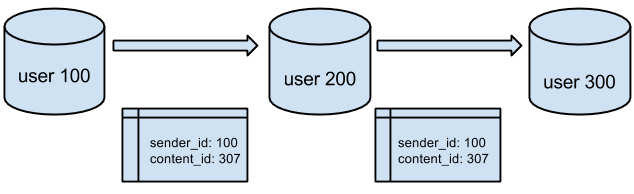
\includegraphics[width=0.8\textwidth]{img/indirection.png}
    \caption{Diagram demonstrating the use of a multi-hop peer-to-peer network to avoid user traffic tracking.
    Since user 100 contacts user 300 via user 200, no direct correlation between user 100 and user 300 can be made
by a third party analysing user 100's traffic.}
    \label{fig:multi-hop}
\end{figure}

There is a possibility of a compromise of reader privacy when a user receives the contents of a web-page which
they wish to view. If a malicious third party (such as their Internet Service Provider, or a rogue user on their
network) were to intercept a user's traffic, they could potentially view the web-content that a user has requested.
The malicious user could then use this information to violate the user's privacy.
To prevent this attack, we can encrypt the web content sent in responses to request for web-page data. Thus, any
attacker that can intercept user traffic could only see encrypted data, and not the actual content that a user has
requested.

\subsubsection{Cryptography}

Each web-page in the system consists of three components apart from its content:
\begin{enumerate}
    \item A randomly generated unique identifier (called a UUID) which identifies this web-page in the system.
    \item A ``content location'' which determines this web-page's storage index in the system.
    \item Cryptographic keys which will be used to encrypt and decrypt web-page data.
We will now briefly discuss these terms and their meanings.
\end{enumerate}

\textbf{UUID}

A web-site's UUID is a unique identifier of this web-page, known only to the users that wish to retrieve it.
These UUIDs are used in the same manner as web URLs, but instead of being in a form similar to a traditional web-site
(for example, www.example.com), they appear as a random string of alphanumeric characters. These identifiers serve
only to identify the web-site and play the same role as a URL in the web as it exists today. These UUIDs could be
shared outside of the system, or they could be linked from another web-page in the system such as a search engine or
web-page indexing site, similar to the case with traditional URLs.

A web-page's UUID is used to derive both its content location and cryptographic keys. These transformations are one-way,
and it should not be possible to derive a web-page's UUID from either its content location nor cryptographic key.

\textbf{Content Location}

A web-page's ``content location'' is a numeric value which determines the ideal node ID in the network at which this content
should be stored. The content location is derived from a web-page's UUID through a hashing function which transforms this unique
identifier into numeric index in the network at which the content should be stored.

It is not guaranteed that a user with any given Node ID will be present on a network. As a result of this, the content should be
stored at the numerically closest node or nodes to the content location identifier.

\textbf{Cryptographic Key}

In order to avoid compromise of user privacy through traffic analysis by malicious third parties, web content being sent to users
on the network should be encrypted. The encryption of this data requires a cryptographic key.

It would be inconvenient for users of the system to hold a database of cryptographic keys relating to web-sites. It would also be
complicated for users to have to manually send cryptographic keys when sharing UUID links to other users. To avoid this, we can
derive cryptographic keys from the web-page's own UUID.

A Key Derivation Function is a cryptographic function that takes an arbitrary string and can
deterministically generate a cryptographic key from it ~\cite{kdf}. Using a Key Derivation Function, we
can generate cryptographic keys to encrypt and decrypt web-page content using only a web-site's UUID.
When sending a request for a web-page, a user must only reveal a hash of its UUID (in order to
find its content location). This means that the only information about user a request that is leaked to the network
is the content location of that web-site. Since it is not possible to derive either the web-page UUID nor the web-page
encryption key from this content location, it is impossible for other users on the network to determine what content
a user is consuming or what UUID this encrypted data represents.

\begin{figure}[H]
    \centering
    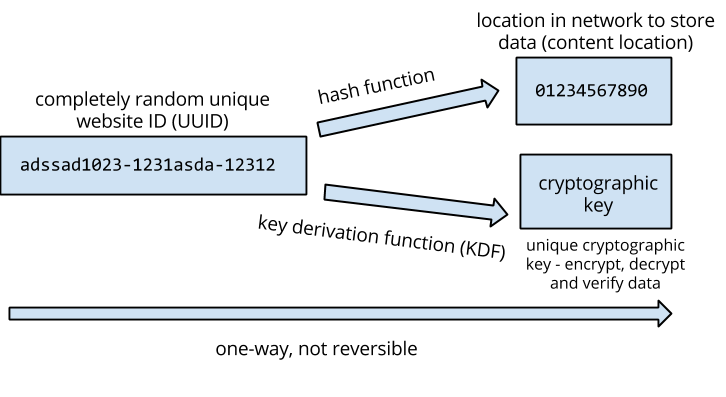
\includegraphics[width=0.8\textwidth]{img/KDF-hashing-example.png}
    \caption{Diagram of the derivation of the content-location and cryptographic key from a web-page UUID.}
    \label{fig:kdf_hashing}
\end{figure}


\subsubsection{Random Sender ID Replacement for Query Anonymity}

It is possible for a malicious user to join the network with the intention of analysing the
sender and destination ID fields in packets that they route through the network. All content request
packets routed through the network include both a sender ID and content ID field.

In Levacher's paper on ``Elite'' ~\cite{levacher}, he introduces a novel way of addressing this issue which we will borrow
in this system.
All users, when passing a request on towards the destination, can randomly change the sender ID field in that message
to their own user ID. When this user receives a response to this modified request, they can simply pass the response
on to the user that originally requested it. This means that users in the network can not reliably tell
the real origin of a request, meaning that none of the users in the system can accurately record the activity of other users.
This concept is demonstrated in figure \ref{fig:sender_id}.

\begin{figure}[H]
    \centering
    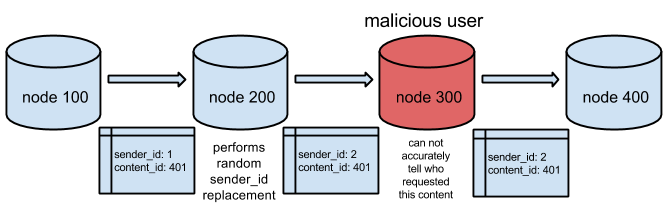
\includegraphics[width=0.8\textwidth]{img/sender_id.png}
    \caption{Diagram demonstrating the usage of random sender ID replacement used to hide the origin of a data request.}
    \label{fig:sender_id}
\end{figure}

%%%%%%%%%%%%%%%%%%%%%%%%%%%%%%%%%%%%%%%%%%%%%%%%%%%%%%%%%%%%%%%%

\subsection{Data Storage}


In order to preserve document anonymity, a user holding some data must not know what the data that they are storing represents.
In the case of this system, this means that a user must not know the UUID of said data.
It is also necessary for a user to have no knowledge of the contents of this data, so that they can not be held
responsible for the actions of other users of the system.

Since content can not be held by its author in order to provide author anonymity, it is important that the legitimacy of stored
data can be verified by the users of the system. It must be possible for users to verify that the data which they receive has
neither been tampered with by the user holding it nor the users in the system that delivered the content to them.
We will refer to this guarantee as ``content integrity''.

In this subsection, we will address and discuss these requirements as well as demonstrate techniques to provide them.

\subsubsection{Document Anonymity}

When a user is requested to hold a piece of data, they are told the content ID, and the encrypted web-page data to store.

The content ID of a piece of data is derived from the UUID of that data. To ensure that the UUID of a piece of data
can not be determined, it must be impossible to derive a UUID from a content location given to a user.
Therefore, the hash function used to derive a content ID from a UUID must be sufficiently complex that it would be
computationally infeasible to derive a UUID if given a content ID ~\cite{sha1}.

The data to be stored is encrypted by a cryptographic key derived from the UUID of that data. The only way to determine
the contents of that encrypted data would be to decrypt it with the cryptographic key.
This cryptographic key is derived from the UUID using a Key Derivation Function.

Since it should be computationally infeasible to derive the UUID of a piece of data from the content ID, it is impossible
for a user to determine either the contents of a piece of stored data or the web-page UUID which it represents.

\subsubsection{Content Integrity}

In order to guarantee content integrity, the system must provide a means of verifying that content stored in the system
has not been modified since being generated by the author. We can achieve this goal by using a cryptographic
technique called a Message Authentication Code (MAC).

A Message Authentication Code is a cryptographic technique used for message authentication - that is, it is used to verify
the authenticity of a message ~\cite{hmac}. Given a message M and cryptographic key K, performing a MAC operation on K and
M will generate an authentication code C. If a user modifies M, it is computationally infeasible for a user that does not
hold the secret key K to compute a new MAC for this modified message. Thus, if a user receives a response to a data request and
the MAC check does not verify the integrity of the contents of the received message, then the content must have been tampered
with since its creation by the content's author and is not reliable. This process is demonstrated in figure \ref{fig:hmac}.

\begin{figure}[H]
    \centering
    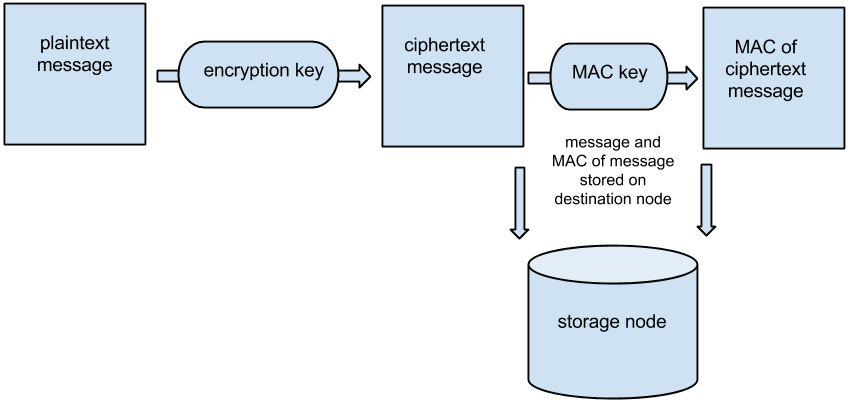
\includegraphics[width=0.8\textwidth]{img/mac.png}
    \caption{A diagram showing the process through which an secure cipher-text (encrypted) message and Message
    Authentication Code for that message is derived from a plain-text (un-encrypted) message.}
    \label{fig:hmac}
\end{figure}


\subsection{Replication}

In order for the system to provide increased reliability and redundancy, data should be
replicated in the network. This will provide resilience against single node failure due to network problems,
disk failure, or other node failure. By adding replication, we aim to remove the single-point-of-failure for a
web-page, providing increased reliability.

Kademlia networks provide automatic content replication ~\cite{kademlia}. In a Kademlia network, there is a
global replication constant among all nodes which determines number of replicas that are kept for any
one piece of data. When some node N leaves the network, the other nodes that hold the replicas of N's data
automatically share the data that N held to the closest available nodes on the network.

We use Kademlia's built-in replication system to provide full document replication in the network.


\subsection{Censorship}

To provide community-driven censorship, the system must allow the users to decide on the censorship of content
on the system.

We will now discuss the difficulties associated with community consensus in a decentralised network and explain the
design choices made in this system to provide community-driven censorship.

\subsubsection{Decentralisation}

Since in this system there is no centralised service providing access to web-pages, access to web-pages can not be
controlled in one place.
Censorship on a web-page can also not be decided by the author of some content as this would enable users to never
have their content censored by the community.
We propose that the censorship of web-pages should be done by the users that hold that web-page data.

\subsubsection{User-based Content Evaluation}

In ``Elite'', Levacher claims that users tend to browse web content that they are generally interested in.
He also argues that if a page is frequently viewed, then it must be of high-quality.

Levacher also makes an argument for a ``Zero-Input Recommendation System.'' Levacher's argument is that evaluating the quality of
content is most effective if users must exert no effort to do so. We argue then that if a users visits a web-page that they do not
object to, then the web-page must be of high quality. This implies that they agree with the content of the web-page and do not deem
it unsuitable for the community. Furthermore, if a user does visit a web-page that they object to, then they are likely to want it to be removed from the system. These users must be given a means to voice their objection to this web-page.

In light of this, we propose a mixture of Levacher's ``Zero-Input Recommendation System'' combined with a channel for users to
report web-pages as unsuitable.
We will allow users to send a notice of objection to a web-page, which we refer to as a ``down-vote''. This phrasing is in the
style of Stack Overflow ~\cite{stackoverflow}. If a user views a web-page and does not send a `down-vote' about this page, then the
system assumes that a user does not object to the content and that the web-page is of high quality.

\subsubsection{``Down-vote''-Based Censorship}

In our system, we propose that censorship be decided by the aggregate ``up-vote'' minus ``down-vote'' value,
where ``up-votes'' are implicitly made when a user does not object to some content.
We will now propose a novel algorithm for the removal of content based on this concept of ``down-votes''.

Data in FreeNet is automatically pruned from the system once is not accessed in some time ~\cite{freenet}.
This serves to remove old and unused content from the network. We will borrow this idea in our system for
the same reason. Web-pages will be given a time-to-live value (TTL), which determines how long until they will
be deleted from the system. Web-page accesses (implicit ``up-votes'') will increase this
TTL, whereas ``down-votes'' will decrease this value, meaning that content will be removed from the network sooner.

\subsubsection{Problems Caused by Kademlia's $\alpha$-Parallelism}

Since the Kademlia network sends messages in parallel to the $\alpha$ closest nodes to a particular destination user ID,
it is entirely possible that a user may receive a single down-vote request twice. This is made worse by the
random sender ID replacement that nodes on the network do to preserve reader anonymity.
This makes it impossible for a user to tell whether they have received a down-vote request more than once.
If we never performed sender ID replacement to down-vote requests, it would compromise reader privacy for the user
sending the down-vote request.

This is mitigated by adding an extra field to down-vote messages: a ``down-vote-UUID'', which is a randomly generated
identifier with which a user can identify a particular down-vote request, and still perform random sender ID
replacement on down-vote requests. We argue that these do not compromise reader anonymity as there is no
user-identifying information present in the down-vote-UUID. If users receives several down-vote requests
with the same down-vote-UUID, they can safely ignore it.

\section{System Design Overview}

\begin{figure}[H]
    \centering
    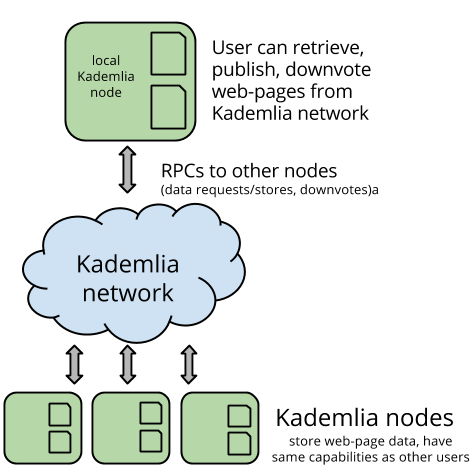
\includegraphics[width=0.6\textwidth]{img/arch.png}
    \caption{A diagram showing the system architecture.}
    \label{fig:arch}
\end{figure}

The system consists of several users (``nodes'') on a Kademlia network. There are three main actions that a user can perform,
with the necessary parameters in brackets:

\subsection{Web-page Retrieval and Verification}

To retrieve a web-page for a given UUID, the user must derive the content location from the UUID using the hash function,
and encryption key and MAC key from the UUID using the Key Derivation Function. They must then retrieve the encrypted data
and MAC from the Kademlia network. They then calculate the expected MAC and compare it to the MAC of the received data. If
they do not match, the data has been tampered with. Otherwise, the user can decrypt the data and read it. This is demonstrated in
figure \ref{fig:retrievalalgo}.

\begin{figure}
    \begin{algorithm}[H]
    \caption{Retrieve web-page from network, given parameter ``UUID''}
    \begin{algorithmic}
        \STATE $content\_location \leftarrow hash(UUID)$
        \STATE $encryption\_key, MAC\_key \leftarrow key\_derivation\_function(UUID) $
        \STATE $actual\_MAC, encrypted\_content \leftarrow kademlia\_lookup(UUID) $
        \STATE $expected\_MAC \leftarrow generate\_mac(encrypted\_content, mac\_key) $
        \IF{$ expected\_MAC \neq actual\_MAC $}
        \RETURN $ error $
        \ENDIF
        \STATE $ decrypted\_content \leftarrow decrypt(encrypted\_content, encryption\_key) $
        \RETURN $ decrypted\_content $
    \end{algorithmic}
    \end{algorithm}
    \caption{Algorithm for retrieving web-page from network.}
    \label{fig:retrievalalgo}
\end{figure}

\subsection{Web-page Publishing}

To publish a web-page, the user must generate a random UUID.
From the UUID, the user then derives the content location using the hash function,
and the encryption and MAC keys using the key derivation function.
They then generate a MAC of the data and the key, and store both of these values at the given content location
in the Kademlia network. This is demonstrated in figure \ref{fig:publishalgo}.

\begin{figure}
    \begin{algorithm}[H]
        \caption{Publish web-page to network, given parameter ``content''}
        \begin{algorithmic}
        \STATE $ UUID \leftarrow generate\_UUID() $
        \STATE $ content\_location \leftarrow hash\_function(UUID) $
        \STATE $ encryption\_key, MAC\_key \leftarrow key\_derivation\_function(UUID) $
        \STATE $ encrypted\_content \leftarrow encrypt(content) $
        \STATE $ MAC \leftarrow generate\_mac(encrypted\_content, mac\_key) $
        \STATE $ kademlia\_store\_value(content\_location, encrypted\_content, MAC) $
        \RETURN $ UUID $
        \end{algorithmic}
    \end{algorithm}
    \caption{Algorithm for publishing web-page to network.}
    \label{fig:publishalgo}
\end{figure}

\subsection{``Down-vote'' Content Censorship Algorithm}

``Down-vote'' messages are passed through the network in the same manner as data retrieval requests. This new request is
not present in the Kademlia specification, and requires modification to any current Kademlia implementations.
The ``down-vote'' Kademlia message simply contacts the nodes holding the data for a given UUID by
using a modified version of the Kademlia content-retrieval remote procedure call (RPC). The user determines the
content-location of this UUID by using the hash function, and then sends this ``down-vote'' RPC to the nodes
responsible for this content location.

Content ``down-votes'' are handled by users storing the data on the network. Users hold three pieces of information about each piece of data they store:
\begin{enumerate}
    \item The data itself.
    \item The aggregate rating of that data, calculated from the number of retrievals minus the number of
    down-votes that the data has received.
    \item A ``time-to-live'' (TTL) value, which represents the time in seconds until the content will be removed from the network.
\end{enumerate}

When a user receives a down-vote request for a piece of data they they are storing, they increment its down-vote counter.
Once every second, every data item's time-to-live value is decreased by a function of their aggregate rating.
While an item's rating is above zero (that is, that its number of up-votes is larger than its number of down-votes),
its TTL does not expire, meaning that highly-rated and often-accessed pages are kept on the network.
Conversely, low-rated pages will eventually be dropped from the network.

\subsubsection{Abuse}

Since down-vote messages are designed to be anonymous, it is possible for users to attempt to cheat the system and
down-vote some content repeatedly until it is removed from the network. This can be stopped in the logic of the
user's application, but this would be an unsatisfactory solution as it would be trivial for the user to circumvent this by
modifying the source of their application, or building a customised client. As a result, there is a trade-off between absolute
anonymity and accurate censorship. We aim to mitigate abuse somewhat in the down-vote algorithm that we use, but our choice was 
to prioritise anonymity over the possibility for abuse.

To counter-act possible abuse by users of the system, our down-vote algorithm decreases a web-page's time-to-live only 
logarithmically as its rating decreases. One per second, we decrease each web-page's time-to-live by a function of its
aggregate rating. This function takes the logarithm of the aggregate rating and subtracts that value, in seconds,
from that value's TTL. As a result, pages with few aggregate down-votes will decay from the network at a slower rate than
those with very large aggregate down-votes. A listing of the algorithm can be found at figure \ref{fig:downvotealgo} for clarity.

Since content is replicated across several nodes on the network by Kademlia, a malicious user would need to send sufficient
down-vote requests to all replicas responsible for some content to completely remove it from the network.
At every second, if a web-page's aggregate score is below zero, then the TTL is decreased by a logarithmic
function of the aggregate score of that web-page, given as:
\[ TTL \leftarrow TTL - log2(absolute\_value(aggregate\_score)) \] 
Thus, the number of down-votes required to remove this content from the network from one replica immediately
(assuming that all requests hit the same replica) would be: $ 2^{TTL} $, as $ TTL - log2(2^{TTL}) = TTL - TTL = 0 $
Since data is replicated in the network by a replication factor, this number becomes $ 2^{TTL} * R $
where $R$ represents the number of replicas serving that piece of web content.
This means that content that was recently added to the network (thus having a high TTL), will be difficult for one
user to remove from the network by virtue of the large number of down-vote requests that they would have to make.
This also assumes that no other user is accessing the content: indeed, if other users are accessing this web-page and
not down-voting it, more requests will be required.

\begin{figure}
    \begin{algorithm}[H]
        \caption{Calculate new TTL for a web-page, given parameters `rating' and `TTL'}
        \begin{algorithmic}
        \IF { $ rating \ge 0 $ }
        \RETURN { $ TTL $ }
        \ENDIF
        \STATE $ score \leftarrow absolute\_value(rating) $
        \STATE $ TTL\_delta \leftarrow log2(score) $
        \RETURN $ TTL - TTL\_delta $
        \end{algorithmic}
    \end{algorithm}
    \caption{Algorithm for calculating a web-pages new TTL, given its current rating and TTL.}
    \label{fig:downvotealgo}
\end{figure}


% Chapter 4:
\chapter{Implementation}

Now that we have discussed the design of our system, we will discuss its implementation.
This design will consist of two main parts:

\begin{enumerate}
	\item{Identical Kademlia user nodes which will make up the Kademlia network.
	The code for these nodes will contain implementation for content look-up, publishing and down-voting and will provide 
	a high-level interface for interfacing with the system. }
	\item A user-facing front-end which will have the ability to look-up content, publish content and down-vote content.
\end{enumerate}

We will first discuss general implementation details, then turn our attention to the implementation of these parts.

\section{The Python programming language}

The project was written using the programming language Python. Python is a high-level interpreted programming language with
light syntax and ``duck-typing'', making it ideal for rapid development. Python also has many useful libraries available,
many of which are open-source under permissive licenses. While none of these factors were essential to the development
of the project, the availability of Python libraries helped with the implementation of the system.

\section{Kademlia Implementations}

While there are several available Python implementations of the Kademlia DHT, many are incomplete or badly documented.
We will discuss the available implementations and their relative advantages and disadvantages.

\subsection{Entangled}

Entangled is a working implementation of the Kademlia DHT written in Python. It provides a high-level programming interface and
a graphical interface for interfacing with the Kademlia network with the ability to demonstrate file-sharing graphically.
Entangled also includes an extra ``delete'' RPC which could be easily modified to serve the purpose of the ``down-vote'' RPC
that our system requires. However, Entangled lacks comprehensive documentation and has a complicated API.
Entangled's code-base is complicated and difficult to understand in places. For this reason, it was decided that Entangled
was not suitable to be used for this system.

Entangled is released under the GNU General Public License, v3 (GPLv3).

\subsection{``Kademlia'' Library}

``Kademlia'' is a Kademlia DHT implementation in Python. ``Kademlia'' seems to be well-documented and written,
but as its first release was published after the beginning of this project, it was decided that it would be too unstable of
a platform to base the project on.
However, the library looks promising and it would be possible for it to be used in future projects once the code-base
has become stable.

``Kademlia'' is released under the MIT license.

\subsection{PyDHT}

PyDHT is a pure Kademlia DHT implementation written in Python. PyDHT does not add extra functionality to the DHT, and its code
is simple enough to be understood, despite its lack of documentation. The code-base of PyDHT is small and modular, making
it possible to easily change the implementation in places. PyDHT includes simple code examples demonstrating how to use the
library. As a result, it was decided that PyDHT would be a suitable base to work on for this project.

PyDHT is released under the BSD 2-clause license.

\subsection{Choice of Kademlia implementation}

It was decided that PyDHT would be used as the base of this project due to its stability, simple API and permissive license.
Since PyDHT is licensed under the 2-clause BSD license, we have forked the library and the modified library will be made
available under the same 2-clause BSD license. The modified library will be made available in Appendix 1.

\section{Cryptography}

\subsection{Key Derivation Functions \& MAC}

The implementation of key-derivation functions and MAC used in the project is written using the PyCrypto Python cryptography library ~\cite{pycrypto}.
The code for this implementation is based on PyCrypto code examples released in to the public domain by Brendan Long ~\cite{kdfexample}.
PyCrypto was chosen due to its proven stability and usage as well as it having functional examples of Key-Derivation Functions.

The key-derivation function chosen to be used for this project was PBKDF2. PBKDF2 was written by RSA labs to replace an earlier standard,
PBKDF1, which could only produce keys with length of up to 160 bits ~\cite{kdf}. PBKDF2 is suitable due to it supporting the generation of
larger keys than 160 bits. This ensures that key-sizes can be increased beyond 160 bits in the future if necessary.
PBKDF2 was chosen due to a readily available implementation being included in the PyCrypto library.
Other key-derivation functions that supported large key-sizes would also be suitable for usage in this system.

The MAC algorithm which was chosen to be used for this project was Hash-based Message Authentication Code (HMAC). HMAC was chosen due to a readily
available implementation being provided in the PyCrypto library and due to it being well-known and proven in the field.
Other MAC algorithms would also be suitable in its place.

\subsection{Hashing function}

The hashing function chosen to be used to derive content locations from UUIDs in the system was SHA-1. This could be replaced with any hashing function
that provided a relatively large key-space. SHA-1 was chosen due to an implementation in the Python standard ``hashlib'' library.

\subsection{Cryptographic keys}

Cryptographic keys are necessary to provide encryption and decryption of data stored by nodes on the network. In order to ensure document anonymity,
the encryption scheme used must be strong enough that it would be infeasible for a node on the network to break it in a reasonable amount of time. The user that publishes some data must be able to encrypt that data, and also allow users to decrypt it.

During the design of the system, we considered both symmetric key encryption and asymmetric key (public-private key) encryption.

Asymmetric-key RSA encryption was initially used for encryption and decryption of content. In RSA, a private-key is used for 
decryption and a public-key for encryption ~\cite{rsa}. Since the system requires that the author encrypts a piece of data and readers decrypt it, the private key would have to be given to users to decrypt web-page data. As a result, asymmetric-key
encryption was decided to be unsuitable for the system.

Symmetric-key encryption uses one cryptographic key for both encryption and decryption. This fits the requirements of our design
specification - the content author and content reader can both use the same cryptographic key for encryption and decryption.
This implementation of the system uses Rijndael AES as its implementation of symmetric-key encryption due to its availability
in the PyCrypto library ~\cite{pycrypto}. Rijndael AES was arbitrarily chosen as it has been proven by its industry use, and had no obvious disadvantage compared to the other algorithms.

\section{Code Structure}

The code is split into two major components, as mentioned previously:
\begin{enumerate}
	\item{A Kademlia-based peer-to-peer network. Since the project uses the PyDHT Kademlia implementation library as a base, most of the code is contained in a modified version of PyDHT.
	This part of the code will provide a Python interface to publish, retrieve and down-vote web-pages as well as handling communication with the underlying Kademlia network.}
	\item{The user-facing front-end code. This part of the code will provide a user interface which will allow a user to publish, retrieve and down-vote web-pages
	on the network. This part of the code-base be composed of two parts:
		\begin{enumerate}
		    \item A Python-based program which will relay messages from the user interface to the underlying modified Kademlia network.
			\item A web-browser-based application which provides a user interface to the network. This will be written in HTML and JavaScript, using web-sockets to communicate
			with the Python program which in turn communicated with the Kademlia network.
		\end{enumerate}
	}
\end{enumerate}

We will now continue to discuss the implementation of both of these components.

\subsection{Kademlia-based Peer-to-Peer Network}

This part of the code is heavily based upon PyDHT, which provides a working Kademlia network as a base on which we build the extra features needed by our network.

\subsubsection{Content Publishing  - \texttt{publish(content)}}

Content publishing is done according to the algorithm described in figure \ref{fig:retrievalalgo}, in the Design section of this paper. This is done in the
publish() function of the DHT class in the source file pydht.py. The function generates a random UUID using the standard Python ``uuid'' library, then derives
the content-location using SHA-1 as the hash function. The function then uses the do\_encrypt() function from the key\_derivation module
to encrypt the data, using the UUID, then stores it in the Kademlia network and returns the UUID.

\subsubsection{Content Retrieval - \texttt{retrieve(uuid)}}

Content retrieval is done according to the algorithm described in figure \ref{fig:publishalgo}, in the Design section of this paper. This is done in the
retrieve() function in the DHT class in the source file pydht.py. The retrieve() function takes the given UUID, and uses the hash function to derive the
content-location. The function then retrieves this content from the Kademlia network, and tries to decrypt it using the do\_decrypt() function from the
key\_derivation module, using the UUID. If either the decryption or MAC checking fails, then the function throws an error. Otherwise, the decrypted data
is returned to the user.

\subsubsection{Encryption \& Key Derivation}

The encryption and key-derivation logic of the system is contained in a key\_derivation Python module which was added to PyDHT. The encryption and decryption functions
written in this module are based on code examples released into the public domain ~\cite{kdfexample}.

This module is comprised of the following functions:

\begin{itemize}
	\item {\texttt{make\_key()} \\
	This function takes a UUID and uses a key-derivation function to generate a cryptographic key.
	This key can then be used to as an AES or HMAC key.
	}
	\item {\texttt{make\_hmac()}\\
	This function takes a message and a cryptographic key and uses the key to create a HMAC verification code of
	the message. This HMAC verification code can then be used for message authentication.
	}
	\item {\texttt{encrypt()}\\
	This function takes a message and a cryptographic key and uses the key to encrypt the message using AES.
	}
	\item {\texttt{decrypt()}\\
	This function takes an encrypted message and a cryptographic key and attempts to decrypt the message using the key.
	An error is thrown if this is unsuccessful.
	}
	\item {\texttt{do\_encrypt()}\\
	This is a simple wrapper function that takes a UUID and a message and returns an encrypted message and HMAC verification code. This function uses
	make\_key to generate an AES key and a HMAC key using the UUID, then encrypts the data and generates a HMAC verification code.
	}
	\item {\texttt{do\_decrypt()}\\
	This is a simple wrapper function that takes a UUID and encrypted message and attempts to decrypt and verify it.
	The function generates a HMAC key and an AES key using make\_key, then attempts to decrypt and verify the encrypted data using them.
	If the verification or decryption fails, the function throws an error. Otherwise, decrypted data is returned.
	}

\end{itemize}

\subsubsection{``Down-vote'' Content Censorship Algorithm}

Down-vote handling is done in the logic of the DHT class. The DHT class keeps a record of the TTL and aggregate down-vote count for each of the pieces of
data that it holds. Once per second, the \texttt{tick()} function is called, which adjusts the TTL of items according to their rating. Once an item's TTL
is less than zero, it is deleted from the network. Figure \ref{fig:code-downvote} shows a code listing taken from the tick() function from the
program source, demonstrating the down-vote algorithm's implementation.

\begin{figure}[H]
	\begin{lstlisting}
for (uuid, rating) in self.webpage_ratings.items():
	if rating < 0:
	    downvote_val = math.log(rating, 2)
	    self.ttls[uuid] -= downvote_val
for (uuid, ttl) in self.ttls.items():
    if ttl <= 0:
        print "UUID", uuid, " past TTL - deleting"
        del self.data[uuid]
	\end{lstlisting}
    \caption{Code listing demonstrating how an item is selected for deletion based on its downvote rating.}
    \label{fig:code-downvote}
\end{figure}

\subsection{User-facing front-end}

As mentioned previously, the front-end is made up of of a JavaScript and HTML web-based front-end, and a Python program which
interfaces with the modified Kademlia network. We will now discuss both of these.

\subsubsection{Browser code - \texttt{websocket-client.html}}

The browser code consists of a simple HTML page which provides inputs for users to open pages for a given UUID, to publish pages,
and to down-vote a page that is currently loaded. The page uses JavaScript to draw requested pages to a section of the browser screen,
sending requests to a local Python interface to the Kademlia network using the JSON serialisation format over a web-socket connection.

\subsubsection{Local node - \texttt{websocket-node.py}}

The Python ``local node" provides the web-based front-end an interface to the Kademlia network. The node simply listens on a web-socket connection
and then relays any requests to the underlying Kademlia network.

The web-socket Python code was adapted from an example in the source code of the AutobahnPython project ~\cite{websocket}, which is released
under the Apache license.

\begin{figure}[H]
    \centering
    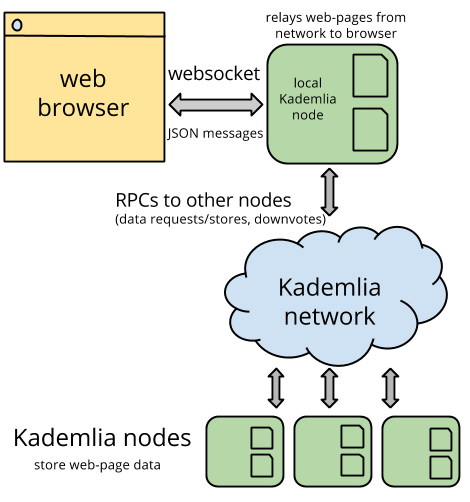
\includegraphics[width=0.6\textwidth]{img/arch-frontend.png}
    \caption{A diagram showing the system architecture, including the user-visible front-end.}
    \label{fig:arch-frontend}
\end{figure}

\subsection{Demonstration shell \& Python scripts}

In order to demonstrate the running of the program, a shell script was included with the project in the
file \texttt{src/demo.sh}.
The script does the following:
\begin{enumerate}
    \item {Creates an initial node that starts the Kademlia-based network}
    \item {Opens ten instances of the xterm terminal emulator which start other nodes
        which then join the network. Messages received by these nodes from the network
        are printed in real-time.}
    \item {Opens a `front-end' node, which listens on a web-socket connection for the front-end.
        This node also joins the Kademlia-based network as a normal user.}
    \item {Opens the web front-end in the Firefox browser. A user can then store and retrieve
        web-pages in the network, and down-vote them.}
\end{enumerate}

This shell script is designed to run on GNU/Linux and has not been tested in other environments.

As well as this shell script, two files \texttt{create\_network.py} and \texttt{join\_network.py}
are provided to create a network and join nodes to it.


% Chapter 4:
\chapter{Future Work}

We will now discuss possible future developments for this project, mentioning the most
interesting areas for improvement.

\section{Censorship}

It was determined over the course of the project that there was a trade-off to be made between complete
reader anonymity and accurate censorship. Indeed, if all requests made in the network
are entirely anonymous, then it becomes difficult to prevent abuse by users that
aim to force censorship on certain content. The design of the content-removal algorithm
proposed in Chapter 3 of this report aims to mitigate this possibility for abuse
by using a logarithmic algorithm for content removal. For future work in this
topic, it would be useful to experiment with this algorithm and the values used by
it on a large-scale, which was unfortunately not possible in the short period in which this
project was done.

\section{Cryptography}

Further research into the cryptography used by the system could prove useful.
Homomorphic encryption, for example, is currently not a feasible approach to this problem due to
the complexity involved in using it. As it is developed further and extended to work
in real-time, it could be used to transform encrypted data in transit between nodes.
This could allow for a more optimal encryption scheme for messages between
users on the network.

\section{Exploits}

It would be particularly interesting to investigate possible exploits present in the
system. One such exploit is related to the use of a symmetric-key for encryption,
decryption and MAC calculations. Since this symmetric key is given to users that read
some data on the network, it would be possible for arbitrary users to calculate new
MAC values for data that they retrieve. This attack would only be useful if a user
knew the UUID of a web-page that they wished to exploit, which means that it could
not be performed by a user to exploit the data that they hold, simply because they
would need to brute-force reverse a known content location to a UUID, which would
require for SHA-1 an average of $2^{160} / 2$ SHA-1 calculations.
This potential exploit could be remedied by the use of some cryptographic scheme where
readers would decrypt with a public key, and authors would encrypt (and calculate MACs)
with a different private key.

\section{User Interface}

For realistic use of the system, a more full-featured user front-end would be required.
While the current prototype works well for single pages, a full alternative web-browser
or browser plugin would provide a much better user experience and would allow for easy
inter-page linking and the embedding of content within other pages (such as external
CSS or JavaScript files). The current front-end only provides a prototype, and extra
time spent developing a user-facing application would be useful. Still, the prototype
front-end developed was not the main focus of the project, and the prototype works
well.

\section{Partial File Replication}

More research info the possibility for partial file replication could prove to be
very interesting. Some large, distributed data-stores that have been developed in the
``Big Data'' industry, such as Google's GFS use a ``sharding'' technique, where stored data
is split into ``chunks'' of a particular size and these chunks are distributed across storage
nodes in the network ~\cite{gfs}. These chunks could be partially redundant: one could imagine a system with
$N+2$ chunks (for example), where only $N$ chunks would be necessary to re-assemble
the original piece of data. This would also save on disk space, and make exploits
on the system more difficult as no single user holds an entire web-page.

\section{Other Applications Based on this System}

It would be interesting to research other possible uses apart from web-serving for the goals
achieved in the design of this system. For example, it would be possible
to adapt the system to serve as the base for an anonymous micro-blogging platform where
user consensus was used to prioritise highly-rated content over poorly-rated content.
In such a system, the global default ``TTL'' could be set to a low value, such as
one hour, and thus only a small amount of the most popular content would remain on the network.

\chapter{Conclusions}

As mentioned in the Introduction to this report, the main goals of this report were
to provide a decentralised web-serving network providing the following guarantees:

\begin{enumerate}
    \item{Decentralisation}
    \item{Author Anonymity}
    \item{Reader Privacy}
    \item{Community-Driven Censorship}
    \item{Increased Reliability and Redundancy}
    \item{Secure Data Storage}
\end{enumerate}

These goals were met, and a successful and functional prototype of a peer-to-peer
network was developed. As well as this, a prototype user-facing front-end which would allow
users to easily interface with the network.

The project was also successful in these other ways:

\begin{enumerate}
	\item { The project implementation was written in a popular, cross-platform programming
	language, Python. Apart from the Linux-specific shell scripts used exclusively for
	project demonstrations, the rest of the client implementation should run on any platform
	which runs Python. This means that the application should run on all popular operating systems,
	widening the possible scope for further development and usage of the project.
	}

	\item{ The web-socket-based ``front-end'' node described in the Implementation section of
	this report allows for user-facing clients to be written in any programming language
	which supports web-sockets and JSON message serialisation.
	This could be used, for example, in an environment such as an Android mobile phone. 
	In such a scenario,  a local Python application can be run
	in the background, and a native Android front-end browsing application could communicate with
	the Python node over web-sockets to access the underlying peer-to-peer network.
	}

    \item{ While this project's main focus was on web-serving, the general principles behind
            community-driven censorship could be used as a base for other types of systems
            that would benefit from community censorship. For example, in our Future Work section,
            we outline ways that the system could serve as a useful base for other applications,
            such as an anonymous micro-blogging platform.
                   }
\end{enumerate}

In answer to the questions set out in this paper's introduction, we conclude that based on the
results of this project that:
\begin{itemize}
    \item Yes, it is possible to build censorship into our system design. Our system
        implementation has demonstrated that this is possible, and achieves censorship
        decided by community decision.
    \item Yes, we can enable censorship by community consensus, but in our system design
        this resulted in a trade-off between the accuracy of this censorship and the
        anonymity of the users. In our system design, we chose to compromise the complete
        accuracy of censorship in order to prioritise complete user anonymity, since user
        anonymity was a primary goal in the system design. However, the system design does
        make abuse difficult, so we argue that the system provides tolerably accurate
        community-driven censorship while still retaining full user anonymity.
\end{itemize}



% insert other chapters here...

% bibliography:
\bibliographystyle{plain}
\bibliography{bib}

\appendix
%%% fokker.tex

\chapter{Code}

All source code for this project has been made publicly available under several open-source licenses.
This source code will be made available on the author's GitHub account, located at
\url{https://github.com/scottcunningham/fyp}, with the exception of the PyDHT fork, which is located
in its own source code repository at \url{https://github.com/scottcunningham/pydht}.

The PyDHT fork located at \url{https://github.com/scottcunningham/pydht} has been released under
the 2-clause BSD License due to the original project's licensing.

The source file in \texttt{pydht/key\_derivation.py} has been released into the public domain since
the code upon which it is based was released as such.

All other code with no explicit license mentioned in the file is released under the Apache license.

% insert other appendices here...

\end{document}
